\textbf{Result: in this set-up PPO did not improve on the tuned prescriptive
rule.} Starting from the rule exactly (residual policy, zero correction),
every PPO update made the noise-free policy \emph{worse} on the
training-period validation windows (Figure~\ref{fig:training}, right).
Checkpoint selection therefore returns update~0, i.e.\ the rule itself, and
the ``PPO'' operation on the test period is identical to the prescribed
functional-flow rule. It is not drawn separately in the figures above.
Scenario~4 (adding hydropower) was not run, since Scenario~3 gave no
learned policy to extend.

\begin{figure}[h]
\centering
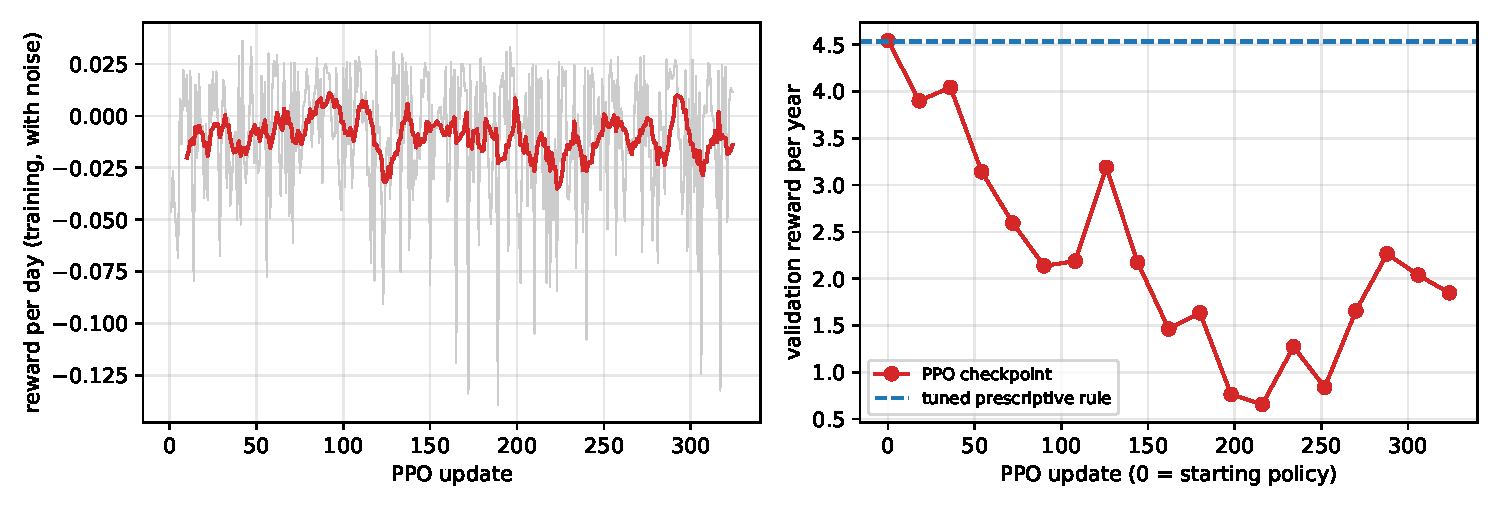
\includegraphics[width=\textwidth]{figures/training_ffreward.pdf}
\caption{Scenario~3 training. Left: mean reward per simulated day of the
noisy training policy (gray: per update; red: 10-update mean). Right: mean
reward per year of each saved checkpoint, run without noise on the five
training-period validation windows, against the tuned prescriptive rule
(dashed). Update 0 is the rule with zero correction.}
\label{fig:training}
\end{figure}

What PPO changed is clear from the reward components
(Table~\ref{tab:ppo_decomp}). The functional-flow part stayed the same
(score 0.85--0.86 throughout), but the policy released progressively more
river water: up to 19~hm$^3$/yr more than the rule. That water was missing
from irrigation in dry years, and the supply term fell from $-4.5$ to
$-7.8$ per year. In other words, the agent paid irrigation water for no
ecological gain.

\begin{table}[h]
\centering\small
\begin{tabular}{@{}lrrrrrrr@{}}
\toprule
 & reward/yr & supply & flood & FF reward & FF score & irrigation [\%] & river [hm$^3$/yr]\\
\midrule
tuned rule & 4.53 & -4.47 & -0.37 & 9.38 & 0.846 & 95.6 & 395 \\
PPO update 72 & 2.59 & -6.32 & -0.43 & 9.35 & 0.858 & 95.1 & 406 \\
PPO update 144 & 2.18 & -6.51 & -0.66 & 9.34 & 0.857 & 95.1 & 407 \\
PPO update 216 & 0.66 & -7.85 & -0.82 & 9.33 & 0.856 & 94.9 & 414 \\
PPO update 324 & 1.85 & -6.66 & -0.74 & 9.25 & 0.853 & 95.1 & 409 \\

\bottomrule
\end{tabular}
\caption{Validation windows (training period): reward components per year
for the rule and for PPO checkpoints.}
\label{tab:ppo_decomp}
\end{table}

\paragraph{Why.} The most likely explanation is a bias that Gaussian
exploration builds into this problem. During training every release
carries random noise (here $\pm4\%$). Near a target, a little extra release
protects the \emph{noisy} policy against falling short. The benefit is
immediate, on the same day, and easy to attribute. The cost (less water
in storage) appears months later, as a hedged irrigation delivery in late
summer or in the next dry year. With $\gamma=0.995$ and three-year
episodes this delayed cost is real in the return, but it is hidden under
much larger random variation between hydrologic years. PPO's advantage
estimates pick up the immediate, noise-protecting benefit and largely miss
the delayed cost. So the policy drifts toward over-releasing, which is the
right reaction for the noisy policy and the wrong one for the deployed,
noise-free policy. The training curve (left panel) shows no clear upward
trend either. The signal that would distinguish a better adaptive rule
from the prescription is small compared with the year-to-year noise.

\paragraph{What the attempts taught.} The path to this result went through
several failures, each instructive (Sections~\ref{sec:reward}
and~\ref{sec:training}):
\begin{enumerate}\itemsep2pt
\item A cloned copy of a calendar-based rule is not the rule. Small action
  errors break day-specific targets, so we learned a correction to the
  rule (residual policy) instead.
\item RL found two reward loopholes within minutes of training: near-miss
  pulse credit that could be collected indefinitely, and double payment
  when the year type changed. Every reward term needs an explicit bound.
\item A reward that differs from the evaluation score gets optimized
  instead of the score. A squared baseflow penalty let PPO shave
  baseflows. The final reward is the daily increment of the score.
\item Pass/fail ecological thresholds on daily flows, and recession limits
  on raw daily changes, make the reward hypersensitive to the exploration
  noise that policy-gradient methods rely on.
\end{enumerate}
